\chapter{Biblioteka: Incremental MST}
\label{app:takeMeHome}
\thispagestyle{appendixStyle}

% Folder tree %%%%%%%%%%%%%%%%%%%%%%%%%%%%%%%%%%%%%%%%%%%%%%%%%%%%%%%%%%%%%%%%%%%%%%%%%%%%%%%%%%%%%%%%%%%%%%%%%%%%%%%%%%

\dirtree{%
.1 /.
.2 \textsc{\textcolor{lgray}{Presentations}}.
.2 \textsc{\textcolor{lgray}{References}}.
.2 \textsc{Scripts}.
.2 \textsc{\textcolor{lgray}{Thesis}}.
.2 \textsc{TMH\_Examples}.
.2 \textsc{TMH\_Library}.
.2 \textsc{TMH\_GraphHelper}.
.2 clear.bash. 
.2 README.md. 
}

\dirtree{%
	.1 /.
	.2 clear.bash \ldots{} 
	\begin{minipage}[t]{5cm}
	\end{minipage}.
	.2 \textsc{Scripts}.
	.3 compileProject.bash \ldots{} 
	\begin{minipage}[t]{5cm}
		Jak omawialiśmy wcześniej~--- służy do kompilacji całego projektu{.}
	\end{minipage}.
	.3 generatePlot.bash \ldots{} 
	\begin{minipage}[t]{5cm}
		Generuje wykresy na podstawie danych, wygenerowanych przez przykładowy program \textsc{TMH\_Examples}{.}
	\end{minipage}.
	.3 makeGraphViz.bash \ldots{} 
	\begin{minipage}[t]{5cm}
		Generuje wizualizację grafu zdefiniowanego w~pliku zgodnym z~opisanym standardem{.}
	\end{minipage}.
}
\newpage

\dirtree{%
	.1 /.
	.2 \textsc{Scripts}.
	.3 randDistance.pl \ldots{} 
	\begin{minipage}[t]{5cm}
		Pozwala na szybką modyfikację wszystkich kosztów ścieżek w~pliku, definiującym graf{.}
	\end{minipage}.	
	.2 \textsc{TMH\_GraphHelper}\ldots{} 
	\begin{minipage}[t]{5cm}
		Pomocniczy projekt do generowania danych wejściowych (napisany w~języku \textsc{Java}){.}
	\end{minipage}.	
}


% OS path %%%%%%%%%%%%%%%%%%%%%%%%%%%%%%%%%%%%%%%%%%%%%%%%%%%%%%%%%%%%%%%%%%%%%%%%%%%%%%%%%%%%%%%%%%%%%%%%%%%%%%%%%%
 \textsf{/Scripts/compileProject.bash}

% Shortcut %%%%%%%%%%%%%%%%%%%%%%%%%%%%%%%%%%%%%%%%%%%%%%%%%%%%%%%%%%%%%%%%%%%%%%%%%%%%%%%%%%%%%%%%%%%%%%%%%%%%%%%%%%
 \texttt{CRTL + ALT + T}

% Nazwy własne, argumenty %%%%%%%%%%%%%%%%%%%%%%%%%%%%%%%%%%%%%%%%%%%%%%%%%%%%%%%%%%%%%%%%%%%%%%%%%%%%%%%%%%%%%%%%%%%%%%%%%%%%%%%%%%
\textsc{R\_USATest\_DKA}

% ANG %%%%%%%%%%%%%%%%%%%%%%%%%%%%%%%%%%%%%%%%%%%%%%%%%%%%%%%%%%%%%%%%%%%%%%%%%%%%%%%%%%%%%%%%%%%%%%%%%%%%%%%%%%
(ang. \textit{Directed acyclic graph})

% Listing %%%%%%%%%%%%%%%%%%%%%%%%%%%%%%%%%%%%%%%%%%%%%%%%%%%%%%%%%%%%%%%%%%%%%%%%%%%%%%%%%%%%%%%%%%%%%%%%%%%%%%%%%%
\begin{lstlisting}[language=bash]
pcname@user:/Scripts$ bash compileProject.bash
\end{lstlisting}

% Figura %%%%%%%%%%%%%%%%%%%%%%%%%%%%%%%%%%%%%%%%%%%%%%%%%%%%%%%%%%%%%%%%%%%%%%%%%%%%%%%%%%%%%%%%%%%%%%%%%%%%%%%%%%

\begin{figure}[!htbp]
	\null\hfill
	%\includegraphics[width=0.8\textwidth]{Appendix_I/GENERATE-PLOT-bash/a_psfrag.pdf}
	\hfill\null
	\caption{
		Wygenerowany wykres dwóch funkcji dla przykładowego wywołania skryptu \textsc{generatePlot.bash}.
	}
\end{figure}

% Figury %%%%%%%%%%%%%%%%%%%%%%%%%%%%%%%%%%%%%%%%%%%%%%%%%%%%%%%%%%%%%%%%%%%%%%%%%%%%%%%%%%%%%%%%%%%%%%%%%%%%%%%%%%

\begin{figure}[!htbp]
	\null\hfill
	\begin{subfigure}[b]{0.49\textwidth}
		\footnotesize
		\begin{lstlisting}[language=bash]
digraph G {
	rankdir=LR;
	node [shape = circle];
	1 -> 2 [ label = "2"];
	1 -> 3 [ label = "6"];
	2 -> 3 [ label = "3"];
	2 -> 4 [ label = "4"];
	2 -> 5 [ label = "5"];
	3 -> 5 [ label = "1"];
	5 -> 4 [ label = "2"];
}
		\end{lstlisting}
		\caption{}
		\label{fig:graphViz:a}
	\end{subfigure}
	\hfill
	\begin{subfigure}[b]{0.49\textwidth}
		%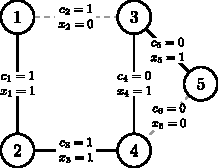
\includegraphics[width=\textwidth]{Appendix_I/GRAPH-VIZ-Example/a.pdf}
		\vspace{1em}
		\caption{}
		\label{fig:graphViz:b}
	\end{subfigure}
	\hfill\null
	\caption{
		Wygenerowana ilustracja grafu przez skrypt \textsc{makeGraphViz.bash}.
		\textbf{(a)}~Kod pośredni pomiędzy danymi wejściowymi w standardowym formacie \textsc{DIMACS Implementation Challenge} a finalnym rysunkiem. Kod pośredni jest zapisany w języku \textsc{DOT}.
		\textbf{(b)}~Rysunek grafu wygenerowany przez program \textsc{GraphViz}.
	}
	\label{fig:graphViz}
\end{figure}

% URL %%%%%%%%%%%%%%%%%%%%%%%%%%%%%%%%%%%%%%%%%%%%%%%%%%%%%%%%%%%%%%%%%%%%%%%%%%%%%%%%%%%%%%%%%%%%%%%%%%%%%%%%%%

\url{http://algs4.cs.princeton.edu/home/} na licencji \textsc{GNU GPLv3}

% ALIGN %%%%%%%%%%%%%%%%%%%%%%%%%%%%%%%%%%%%%%%%%%%%%%%%%%%%%%%%%%%%%%%%%%%%%%%%%%%%%%%%%%%%%%%%%%%%%%%%%%%%%%%%%%

	\begin{align*}
		f(x) +    g(x)  &=          \cos(x) +              \sin(x)             + h(x) \\
		\phantom{f(x) +{}} g(x)  &= \phantom{\cos(x) +{}}          {\sin(x)} \phantom{{}+ h(x)}\\
		f(x)  \phantom{{}+ g(x)} &=          \cos(x) \phantom{{} +  \sin(x)}            + h(x) \\
		s(x)  \phantom{{}+ g(x)} &= \phantom{\cos(x) +{}} \makebox[\widthof{$\sin(x) + h(x)$}][c]{$\arcsin(x)$}
	\end{align*}